\documentclass[11pt]{article}
\renewcommand{\baselinestretch}{1.05}
\usepackage{amsmath,amsthm,verbatim,amssymb,amsfonts,amscd, graphicx}
\usepackage[parfill]{parskip}
\usepackage{graphics}
\usepackage{graphicx}


\topmargin0.0cm
\headheight0.0cm
\headsep0.0cm
\oddsidemargin0.0cm
\textheight23.0cm
\textwidth16.5cm
\footskip1.0cm
\theoremstyle{plain}
\newtheorem{theorem}{Theorem}
\newtheorem{corollary}{Corollary}
\newtheorem{lemma}{Lemma}
\newtheorem{proposition}{Proposition}
\newtheorem*{surfacecor}{Corollary 1}
\newtheorem{conjecture}{Conjecture} 
\newtheorem{question}{Question} 
\theoremstyle{definition}
\newtheorem{definition}{Definition}

\begin{document}	
	
	\title{Data Science Curriculum}
	\author{Daniel Kerim Acatay}
	\maketitle
	
\section{Preface}
This is a scrapped together curriculum of important concepts for the successfull Data Scientist. All contents, visualization as well as documentation, are taken from the collaborative efforts of the scientific communities
\begin{itemize}
	\item https://www.wikipedia.org
	\item http://scikit-learn.org
\end{itemize}
This documented to a margin owed to the great work of to the respective authors and communities. I merely put the contents in an order as I saw fit for the applied work as a data scientist. 

As this is a living document, more contents are added to the curriculum as I learn on the job.

\section{Machine Learning Lingo}
\textit{Artificial Intelligence} (AI) is concerned with the study of intelligent machines that can perform tasks that are characteristic for human intelligence. In that regard, intelligent refers for example to the understanding of human language, recognition of objects and sounds, or solving complex problems. 

\textit{Machine learning} (ML) is the task of teaching a computer system the ability to learn from input data without being explicitly programmed. To put things in perspective, machine learning is a way to achieve artificial intelligence. One could build an AI without the use of ML, however, this would require a vast amount of hard coding of complex decision rules.

\subsection{Learning types}
In general, a learning problem considers a set of $N$ samples of data and then tries to predict properties of new unknown data. If each sample is more than a single number and, for instance, a multi-dimensional entry (aka multivariate data), it is said to have several attributes or features.
\begin{itemize}
	\item Supervised Learning
	\item Unsupervised Learning
	\item Reinforcement Learning
\end{itemize}

\subsubsection{Supervised Learning}
\textit{Supervised Learning} is concerned with finding a mapping function $y=f(x)$ from $N$ labeled training data tuples $\{ (x_i, y_i)\}_{i=1}^N$, where $x_i$ is a $k$-dimensional features vector and $y_i$ is the target or output variable (label / class). In general, we distinguish between two broad classes of supervised learning problems:
\begin{itemize}
	\item Classification problems
	\item Regression problems
\end{itemize}
\textit{Classification} is the problem of identifying to which of a set of categories (sub-populations) a new observation belongs, on the basis of a training set of data containing observations (or instances) whose category membership is known. The target variable is categorical or discrete.

In \textit{regression}, the outputs are continuous rather than discrete.

\subsubsection{Unsupervised Learning}
In \textit{Unsupervised Learning} the training data consists only of a set of feature vectors $x$ without any corresponding target values. The goal of such of inferring a function to describe hidden structure from unlabeled data. Since training examples are unlabelled, there is no evaluation of the accuracy to improve on a predictive model like it is the case with supervised learning methods. We distingusih between three broad categories:
\begin{itemize}
	\item Clustering
	\item Density estimation
	\item Dimensionality reduction is the task of representing data in a lower dimensionality
\end{itemize}

\textit{Clustering} refers to grouping data into categories based on some measure of inherent similarity or distance.

\textit{Density estimation} refers the construction of an estimate, based on observed data, of an unobservable underlying probability density function. The unobservable density function is thought of as the density according to which a large population is distributed; the data are usually thought of as a random sample from that population.

\textit{Dimensionality reduction} is the process of reducing the number of features under consideration by obtaining a set of principal components which explain the most of the data behaviour.

\subsection{Generative vs. discriminative approaches}
\textbf{Discriminative models}  learn the (hard or soft) boundary between classes.

\noindent\textbf{Generative models}  model the distribution of individual classes

\subsection{Curse of Dimensionality}
In machine learning problems that involve learning a "state-of-nature" from a finite number of data samples in a high-dimensional feature space with each feature having a range of possible values, typically an enormous amount of training data is required to ensure that there are several samples with each combination of values. A typical rule of thumb is that there should be at least 5 training examples for each dimension in the representation. With a fixed number of training samples, the predictive power of a classifier or regressor first increases as number of dimensions/features used is increased but then decreases, which is known as Hughes phenomenon or peaking phenomena


\section{The Mathematics Curriculum}
Linear Function linear mapping

\subsection{Eigenvalues nad -vectors of a matrix}
Multiplying a vector by a matrix, $Ax$, usually rotates the vector $x$, however, in some cases of x, $Ax$ is parallel to x, i.e.
\begin{equation}
Ax = \lambda x
\end{equation}
for some $\lambda$. The number $\lambda$ is an \textit{eigenvalue} of matrix $A$, if there exists a vector $x$, such that $A\text{x} = \lambda x$. The vector x is an \textit{eigenvector} corresponding to eigenvalue $\lambda$.

gradients to matrices

complex numbers



\section{The Statistics Curriculum}
\subsection{Probability Density Functions (PDFs)}
A \textit{probability mass function} (PMF) is a function that gives the probability that a discrete random variable is exactly equal to some value. The probability mass function is often the primary means of defining a discrete probability distribution, and such functions exist for either scalar or multivariate random variables whose domain is discrete.

A probability mass function differs from a \textit{probability density function} (PDF) in that the latter is associated with continuous rather than discrete random variables. The values of the probability density function are not probabilities as such: a PDF must be integrated over an interval to yield a probability

The probability of a real-valued scalar variable $x$ is described with its probability density function, $p(x)$, that satisfies
\begin{align}
p(x) \  & \ \geq 0 \qquad \text{for all $x$} \\
\int_{-\infty}^{\infty} p(x) dx \ &= \ 1
\end{align}
The probability that a random variable $x$ falls within a given range is
\begin{equation}
\text{Pr}(a \leq x \leq b) \ = \ \int_{a}^{b}p(x)dx
\end{equation}
A probability density is \textit{not} a probability per se. Moreover, the probability that a continuous random variable $x$ takes on a specific value is always zero, e.g. $P(x=3) = \int_3^3p(c)dx=0$.

The \textit{joint distribution} $p(x,y)$ for two random variables $x$ and $y$ defines the probability that $(x,y)$ lies in a given domain $\mathcal{D}$:
\begin{equation}
\text{Pr}((x,y) \in \mathcal{D}) \ = \ \int_{(x,y)\in \mathcal{D}} p(x,y)dxdy
\end{equation}
For example, the probability the coordinate $(x,y)$ lies in domain $(0\leq x \leq 1,0\leq y\leq 1)$ is calculated by $\int_{0\leq x \leq 1} \int_{0\leq y \leq 1}p(x,y)dxdy$. For a vector $\textbf{a} = \left[x,y\right]^T$ the PDF for $p(\textbf{a})$ is equivalent to $p(x,y)$.

The \textit{conditional distribution} $p(x|y)$ expresses the probability distribution of $x$ for a known value of $y$

Probability rules of PDFs are:
\begin{itemize}
	\item Sum rule: $\int_{-\infty}^{\infty}p(x)dx=1$
	\item Product rule: $p(x,y) = p(x|y)p(y)=p(y|x)p(x)$
	\item Marginalization: $p(y) = \int_{-\infty}^{\infty} p(x,y) dx$
	\item Independence: $x$ and $y$ are independent if $p(x,y)=p(x)p(y)$
\end{itemize}

\subsection{Mathematical Expectation and Variance}
The \textbf{mean} $\mu$ of a density $p(x)$ is the expected value of a random variable $x$
\begin{equation}
\mu= \mathbb{E}[x] \ = \ \int x p(x) dx
\end{equation}
The \textbf{variance} of a scalar variable $x$ is the expected squared deviation from the mean:
\begin{equation}
\mathbb{E}[(x-\mu)^2] \ = \ \int (x-\mu)^2 p(x) dx
\end{equation}
The covariance of a vector \textbf{x} is a matrix
\begin{equation}
\Sigma = \text{cov}\left(\textbf{x}\right) = \mathbb{E}[\left(\textbf{x}-\boldmath{\mu}\right)(\text{x}-\boldmath{\mu})^T] = \int (\textbf{x}-\boldmath{\mu})(\text{x}-\boldmath{\mu})^T p(\text{x}) d\text{x}
\end{equation}
The diagonal entries of the covariance matrix are the variances of the individual entries over the vector
\begin{equation}
\Sigma_{ii} = \text{var}(x_{ii}) = \mathbb{E}[(x_i-\mu_i)^2]
\end{equation}
The off-diagonal terms are \textbf{covariances}
\begin{equation}
\Sigma_{ij} = \text{var}(x_{i},x_{j}) = \mathbb{E}[(x_i-\mu_i)(x_j-\mu_j)]
\end{equation}
between variables $x_i$ and $x_j$.

\subsection{Distributions}

\subsubsection{Bernoulli Distribution}
A \textit{Bernoulli trial} is a random experiment where a random variable has exactly two possible outcomes, $X \in \{0,1\}$. Then, $X$ is said to follow a \textit{Bernoulli distribution}, denoted $X \sim \mathbb{B}(p)$,  with corresponding PDF
\begin{equation}
\text{Pr}(X=k|p) \ = \ p^k(1-p)^{1-k}
\end{equation}
and
\begin{itemize}
	\item $\mathbb{E}[X] = p$
	\item $\text{var}[X] = p(1-p)$
\end{itemize}

\subsubsection{Binomial Distribution}
The probability of getting $k$ successes in $n$ independent Bernoulli trials is described by the \textit{Binomial Distribution}, denoted $Y \sim \mathcal{B}(n,p)$, with corresponding PMF
\begin{equation}
\text{Pr}(X=k|n,p) \ = \ \binom{n}{k}p^k(1-p)^{n-k} \ = \ \frac{n!}{k!(n-k)!} p^k(1-p)^{n-k}
\end{equation}
and
\begin{itemize}
	\item $\mathbb{E}[X] = np$
	\item $\text{var}[X] = np(1-p)$
\end{itemize}
For a single trial, i.e. $n=1$, the binomial distribution is a Bernoulli distribution.

\subsubsection{Poisson Distribution}
The Poisson distribution is a discrete probability distribution that expresses the occurrences of some event over a specified interval. The probability of observing $k$ events in an interval is given by equation
\begin{equation}
\text{Pr}(X=k|\theta) = \frac{\theta^k e^{-\theta}}{k!}
\end{equation}
and
\begin{itemize}
	\item $\mathbb{E}[X] = \lambda$
	\item $\text{var}[X] = \lambda$
\end{itemize}

\subsubsection{Uniform Distribution}

\begin{equation}
\text{Pr}(X=k|p) \ = \ p^k(1-p)^{1-k}
\end{equation}
and
\begin{itemize}
	\item $\mathbb{E}[X] = p$
	\item $\text{var}[X] = p(1-p)$
\end{itemize}

\subsubsection{Normal Distribution}
The Normal distribution, denoted $\mathcal{N}(\mu,\sigma^2)$, has a PDF of form
\begin{equation}
p(x|\mu,\sigma^2) \ = \ \frac{1}{\sqrt{2\pi\sigma^2}} \exp{\left(-\frac{1}{2\sigma^2}(x-\mu)^2\right)}
\end{equation}

The PDF for a $D$-dimensional vector \textbf{x}, the elements of which are jointly normal distributed, denoted $\textbf{x} \sim \mathcal{N}(\boldmath{\mu}, \Sigma)$, is given by
\begin{equation}
p\left(\textbf{x}|\boldmath{\mu},\Sigma\right) \ = \ \frac{1}{\sqrt{(2\pi)^D|\Sigma|}} \exp{\left(-\frac{1}{2}(\textbf{x}-\boldmath{\mu})^T\Sigma^{-1}(\textbf{x}-\boldmath{\mu}\right)}
\end{equation}
An important special case arises when the Gaussian is isotropic (rotationally invariant) and the covariance matrix can be written as $\sigma = \sigma^2\textbf{I}$. This reduces the PDF to
\begin{equation}
p\left( \textbf{x} | \boldmath{\mu} , \sigma^2 \right) \ = \ \frac{1}{\sqrt{(2\pi)^D\sigma^D}} \exp{\left(-\frac{1}{2\sigma^2}||\textbf{x}-\boldmath{\mu}||^2\right)}
\end{equation}

The covariance matrix $\Sigma$ of a Gaussian must be symmetric and positive definite - this is equivalent to requiring $|\Sigma| > 0$. Otherwise, the formula does not correspond to a valid PDF, since equation would no longer be real-valued if $|\Sigma| \leq 0$.


\subsection{Standard Normal Distribution}
For th special case when $\mu = 0$ and $\sigma=1$ the normal distribution is known as \textit{standard normal distribution} with BDF
\begin{equation}
\phi(x) \ = \ \frac{1}{\sqrt{2\pi}} e^{-\frac{1}{2}x^2}
\end{equation}

\subsection{Beta Distribution}
The PDF of the \textit{Beta Distribution}, denoted $X \sim \text{Beta}(\alpha, \beta)$, is defined on the interval $\left[0,1\right]$, with shape parameters $\alpha, \beta > 0$ as
\begin{equation}
p(x|\alpha,\beta) \ = \ \frac{(\alpha + \beta)}{\Gamma(\alpha)\Gamma(\beta)} x^{\alpha-1}(1-x)^{\beta-1} \ = \ \frac{1}{\text{B}(\alpha,\beta)} x^{\alpha-1}(1-x)^{\beta-1}
\end{equation}
where $\Gamma$ is the gamma function and B is the beta function.


\subsection{Gamma Distribution}


\subsection{Inverse Gamma Distribution}



\section{The Baysian Paradigm}
The Bayesian theory of probability is concerened with how information is used to update subjective prior believes. In general, given that we have a model of the world described by a unknown parameter (vector) $\theta$ and observable data \textbf{y}, our goal ist to determine the model, i.e. the unkonwn parameters, from the data.

As is the case in the Bayesian paradigm, the model parameters $\theta$ are found to stem from a \textit{a posteriori} distribution which is the combination of \textit{a priori} knowledge about the model parameters and the likelihood of the data genereating process underlying the observable data.

From the product rule of proability density function we know that
\begin{equation}
p(\textbf{y}, \theta) \ = \  p(\textbf{y}| \theta) p(\theta) \ = \ p(\theta|\textbf{y}) p(\textbf{y})
\end{equation}
This can be rearranged such that we find Bayes' Rule:
\begin{equation}
\underbrace{p(\theta|\textbf{y})}_{\text{posterior}} \ = \  \frac{\overbrace{p(\theta)}^{\text{prior}} \overbrace{p(\textbf{y}| \theta)}^{\text{likelihood}} }{ \underbrace{p(\textbf{y})}_{\text{evidence}}}
\end{equation}
where
\begin{itemize}
	\item the \textit{posterior distribution} describes the knowledge of the population parameter $\theta$, incorporating both the data and the prior knowledge
	\item the \textit{likelihood} describes the data generating process of the observed population,
	\item the \textit{prior distribution} describes our assumption of the unknown population parameter $\theta$ before the arrival of new information through the likelood function,
	\item the \textit{evidence}, or prior predictive distribution, which ensures that the posterior distribution integrates to one.
\end{itemize}
A more expressive notation used throughout will be
\begin{equation}
\pi(\theta|\textbf{y}) \ = \ \frac{p(\theta)\mathcal{L}(\theta;\textbf{y})}{p(\textbf{y})} \ \propto \ p(\theta)\mathcal{L}(\theta;\textbf{y})
\end{equation}
In this representation the term $p(\textbf{y})$, for observable $\textbf{y}$, can be considered a constant ensuring that the posterior density integrates to one.

\section{Linear Regression}
Learn the mapping from one real-valued space to another

\subsection{One dimensional case}
The goal is to learn the mapping $\text{y}=f(\text{x})$, where x and y are scalar real-valued, i.e. $\text{x} \in \mathbb{R}$ and $\text{y} \in \mathbb{R}$. We assume $f$ to have a linear form
\begin{equation}
	\text{y}=w\text{x}+b
\end{equation}
where $w$ is a weight and $b$ is a bias. We want to estimate $w$ and $b$ from $N$ training pairs $\{ (\text{x}_i, y_i)\}_{i=1}^N$. Once we have found $w$ and $b$ we can compute y for new x.

The parameters are estimated using \textit{least squares regression}. Define the \textit{energy function}, or \textit{objective function}
\begin{equation}
E\left(w,b\right) = \sum_{i=1}^N \left(\text{y}_i - \left(w\text{x}_i + b\right)\right)^2
\end{equation}
To estimate $w$ and $b$, we solve for the $w$ and $b$ that minimize $E$. The partial derivative with respect to $b$ is given by
\begin{equation}
\frac{\partial E}{\partial b} = -2 \sum_{i=1}^N \left(\text{y}_i - \left(w\text{x}_i + b\right)\right) = 0.
\end{equation}
Solving for $b$ yields the error minimizing bias estimate $b^*$
\begin{equation}
b^* = \frac{\sum \text{y}_i}{N} - w \frac{\sum \text{x}_i}{N} = \bar{y} - w\bar{\text{x}}.
\end{equation}
Substituting the optimal $b^*$ into the energy equation yields
\begin{equation}
E\left(w,b^*\right)= \sum_i \left(\left(\text{y}_i-\bar{y}\right) - w \left(\text{x}_i - \bar{\text{x}}\right)\right)^2
\end{equation}
Then, solving the partial derivative with respect to $w$ with form
\begin{equation}
\frac{\partial E}{\partial w} = -2 \sum_i \left(\left(\text{y}_i-\bar{\text{y}}\right) - w \left(\text{x}_i - \bar{\text{x}}\right)\right)\left(\text{x}_i - \bar{\text{x}}\right) = 0
\end{equation}
yields the optimal weight parameter $w^*$ with
\begin{equation}
w^* = \frac{\sum_i\left(\text{y}_i-\bar{\text{y}}\right)\left(\text{x}_i-\bar{\text{x}}\right)}{\sum_i\left(\text{x}_i-\bar{\text{x}}\right)^2}
\end{equation}



\subsection{Multidimensional inputs}
The goal is to learn a mapping from $D$-dimensional inputs to a scalar output: $\textbf{x} \in \mathbb{R}^D$, $y \in \mathbb{R}$. For a vector of weights \textbf{w}, the mapping will be
\begin{align}
f\left(\textbf{x}\right) &= \sum_{j=1}^D w_j\text{x}_j +b \nonumber \\
&= \textbf{w}^T\textbf{x} + b \nonumber \\
&=\tilde{\textbf{w}}^T \tilde{\textbf{x}}
\end{align}
where the bias is folded into the vectors
\begin{equation}
\tilde{\textbf{w}} = \begin{bmatrix}
	w_1 \\
	\vdots \\
	w_d\\
	b	
	\end{bmatrix}, \qquad \tilde{\textbf{x}} = \begin{bmatrix}
	\text{x}_1 \\
	\vdots \\
	\text{x}_d\\
	1	
	\end{bmatrix}
\end{equation}
Given $N$ training data pairs, the least-squares objective function is
\begin{align}
E\left(\tilde{\textbf{w}}\right) &= \sum_{i=1}^N \left(y_i - \tilde{\textbf{w}}^T \tilde{\textbf{x}_i} \right)^2 \nonumber \\
 &= ||\tilde{\textbf{y}} - \tilde{\textbf{X}}\tilde{\textbf{w}} ||^2 \nonumber \\
&= (\textbf{y} -  \tilde{\textbf{X}} \tilde{\textbf{w}} )^T (\textbf{y} -  \tilde{\textbf{X}} \tilde{\textbf{w}} ) \nonumber \\
&= \tilde{\textbf{w}}^T \tilde{\textbf{X}}^T \tilde{\textbf{X}} \tilde{\textbf{w}} -2 \textbf{y}^T\tilde{\textbf{X}}\tilde{\textbf{w}} + \textbf{y}^T \textbf{y}
\end{align}
where
\begin{equation}
\tilde{\textbf{y}} = \begin{bmatrix}
y_1 \\
\vdots \\
y_N	
\end{bmatrix}, \qquad \tilde{\textbf{X}} = \begin{bmatrix}
\text{x}_1 & 1\\
\vdots \\
\text{x}_N^T & 1	
\end{bmatrix}
\end{equation}
and $||\cdot||$ is the usual Euclidian norm, i.e. $||\textbf{v}||^2=\sum_i v_i^2$. We find the solution to this by optimizing $E$ with respect to $\tilde{\textbf{w}}$ and solving
\begin{align}
\frac{\partial E}{\partial \tilde{\textbf{w}}} = 2 \tilde{\textbf{X}}^T \tilde{\textbf{X}} \tilde{\textbf{w}} -2 \tilde{\textbf{X}}^T \textbf{y} = 0 
\end{align}
which yields
\begin{equation}
 \tilde{\textbf{w}}  = (\tilde{\textbf{X}}^T \tilde{\textbf{X}})^{-1} \tilde{\textbf{X}}^T \textbf{y}
\end{equation}


\section{Nonlinear Regression}

\section{Supervised Learning}
\subsection{k-Nearest Neighbours}
In pattern recognition, the $k$-\textit{Nearest Neighbors Algorithm} (k-NN) is a non-parametric method used for classification and regression. In both cases, the input consists of the $k$ closest training examples in the feature space. 

\subsubsection{Nearest Neighbor Classification}
In \textit{k-NN classification}, the output is a class membership. An object is classified by a majority vote of its neighbors, where class membership is assigned among the most common among its $k$ nearest neighboring data points. If $k = 1$, then the object is simply assigned to the class of that single nearest neighbor. Similarity is defined according to a distance metric, typically the \textit{Euclidian distance}:
\begin{equation}
d(x,x')=\sqrt{(x_1-x'_1)^2 + (x_2-x'_2)^2 + \dots + (x_N-x'_N)^2}
\end{equation}

Formally, given a positive integer $k$, a new observation $x'$, and a similarity metric $d$, the kNN classifier computes $d$ between $x'$ and each training observation. The set of $k$ data points from the training data that are closest to $x'$ is denoted $\mathcal{K}$. It then estimates the conditional probability for each class, that is, the fraction of points in $\mathcal{K}$ with that given class label.
\begin{equation}
P(y=j|X=x) = \frac{1}{k} \sum_{i \in \mathcal{K}} I(y^{(i)}=j)
\end{equation}
The new observation $x'$ is assigned to the class with the largest probability.


\subsubsection{Nearest Neighbor Regression}
In \textit{k-NN regression}, the output is the property value for the object. This value is the average of the values of its k nearest neighbors. The basic nearest neighbors regression uses uniform weights: that is, each point in the local neighborhood contributes uniformly to the classification of a query point. Under some circumstances, it can be advantageous to weight points such that nearby points contribute more to the regression than faraway points. 



\subsubsection{Dimensionaility reduction}
For high-dimensional data (e.g., with number of dimensions more than 10) dimension reduction is usually performed prior to applying the k-NN algorithm in order to avoid the effects of the curse of dimensionality.

The curse of dimensionality in the k-NN context basically means that Euclidean distance is unhelpful in high dimensions because all vectors are almost equidistant to the search query vector (imagine multiple points lying more or less on a circle with the query point at the center; the distance from the query to all data points in the search space is almost the same).

Feature extraction and dimension reduction can be combined in one step using principal component analysis (PCA), linear discriminant analysis (LDA), or canonical correlation analysis (CCA) techniques as a pre-processing step, followed by clustering by k-NN on feature vectors in reduced-dimension space. In machine learning this process is also called low-dimensional embedding

\subsection{Support Vector Machines  (SVM)}
A support vector machine constructs a hyperplane or set of hyperplanes in a high- or infinite-dimensional space, which can be used for classification, regression, or other tasks like outliers detection[3]. Intuitively, a good separation is achieved by the hyperplane that has the largest distance to the nearest training-data point of any class (so-called functional margin), since in general the larger the margin the lower the generalization error of the classifier.



\subsection{Classification and Regression Trees}
\textit{Decision Trees} are a non-parametric supervised learning method used for classification and regression. 

\subsubsection{Decision Tree Learning}
A decision tree learning algorithm partitions a data set into smaller disjunct sets, the \textit{leaves} or \textit{terminal nodes}, using simple if-else decision rules inferred from the data features.

Given a labeled training sample $\{x_i,y_i\}_{i=1}^N$ with $x_i \in \mathbb{R}^d$ and target $y_i \in \mathbb{R}^N$ a decision tree recursively partitions the data space $\mathcal{X}$ into $l$ disjoint sets $\mathcal{A}_1, \dots,\mathcal{A}_c$, such that the predicted value of $y_i$ is $j$ if $x_i$ belongs to $\mathcal{A}_j$ for $j = 1, \dots, c$.

Let $Q$ denote the data at node $m$. For each candidate split $\theta=(j,t_m)$ with feature $j$ and threshold $t_m$, a decision tree partitions the data into $Q_{left}(\theta)$ and $Q_{right}(\theta)$. The impurity at node $m$ is computed using a impurity function $H(\cdot)$ (depending on classification or regression tree)
\begin{equation}
G(\theta) = \frac{N_{left}}{N_m}H(Q_{left}(\theta)) + \frac{N_{right}}{N_m}H(Q_{right}(\theta)) 
\end{equation}
Select the parameters $\theta^*$ that minimize the impurity
\begin{equation}
\theta^* = \arg\min_\theta G(\theta)
\end{equation}
This is repeated until a stopping criteria is reached, which might be a maximum depth of the tree, or the number of samples in each leaf reaches a threshold.

\subsubsection{Classification criteria}
For a categorical target outcome, let the proportion of observations of class $k$ be
\begin{equation}
p_{mk} = \frac{1}{N_m}\sum_{x_i\in \mathcal{R}_m} I(y_i=k)
\end{equation}
with $\mathcal{R}_m$ representing the region appertaining to node $m$. Most frequent impurity measures are \textbf{Gini impurity} of the form
\begin{equation}
H(\mathcal{X}_m) = \sum_k p_{mk}(1-p_{mk})
\end{equation}
and \textbf{cross-entropy} of the form
\begin{equation}
H(\mathcal{X}_m) = \sum_k p_{mk}\log(p_{mk})
\end{equation}
where $\mathcal{X}_m$ is the training data in node $m$.
\begin{figure}[h!]
	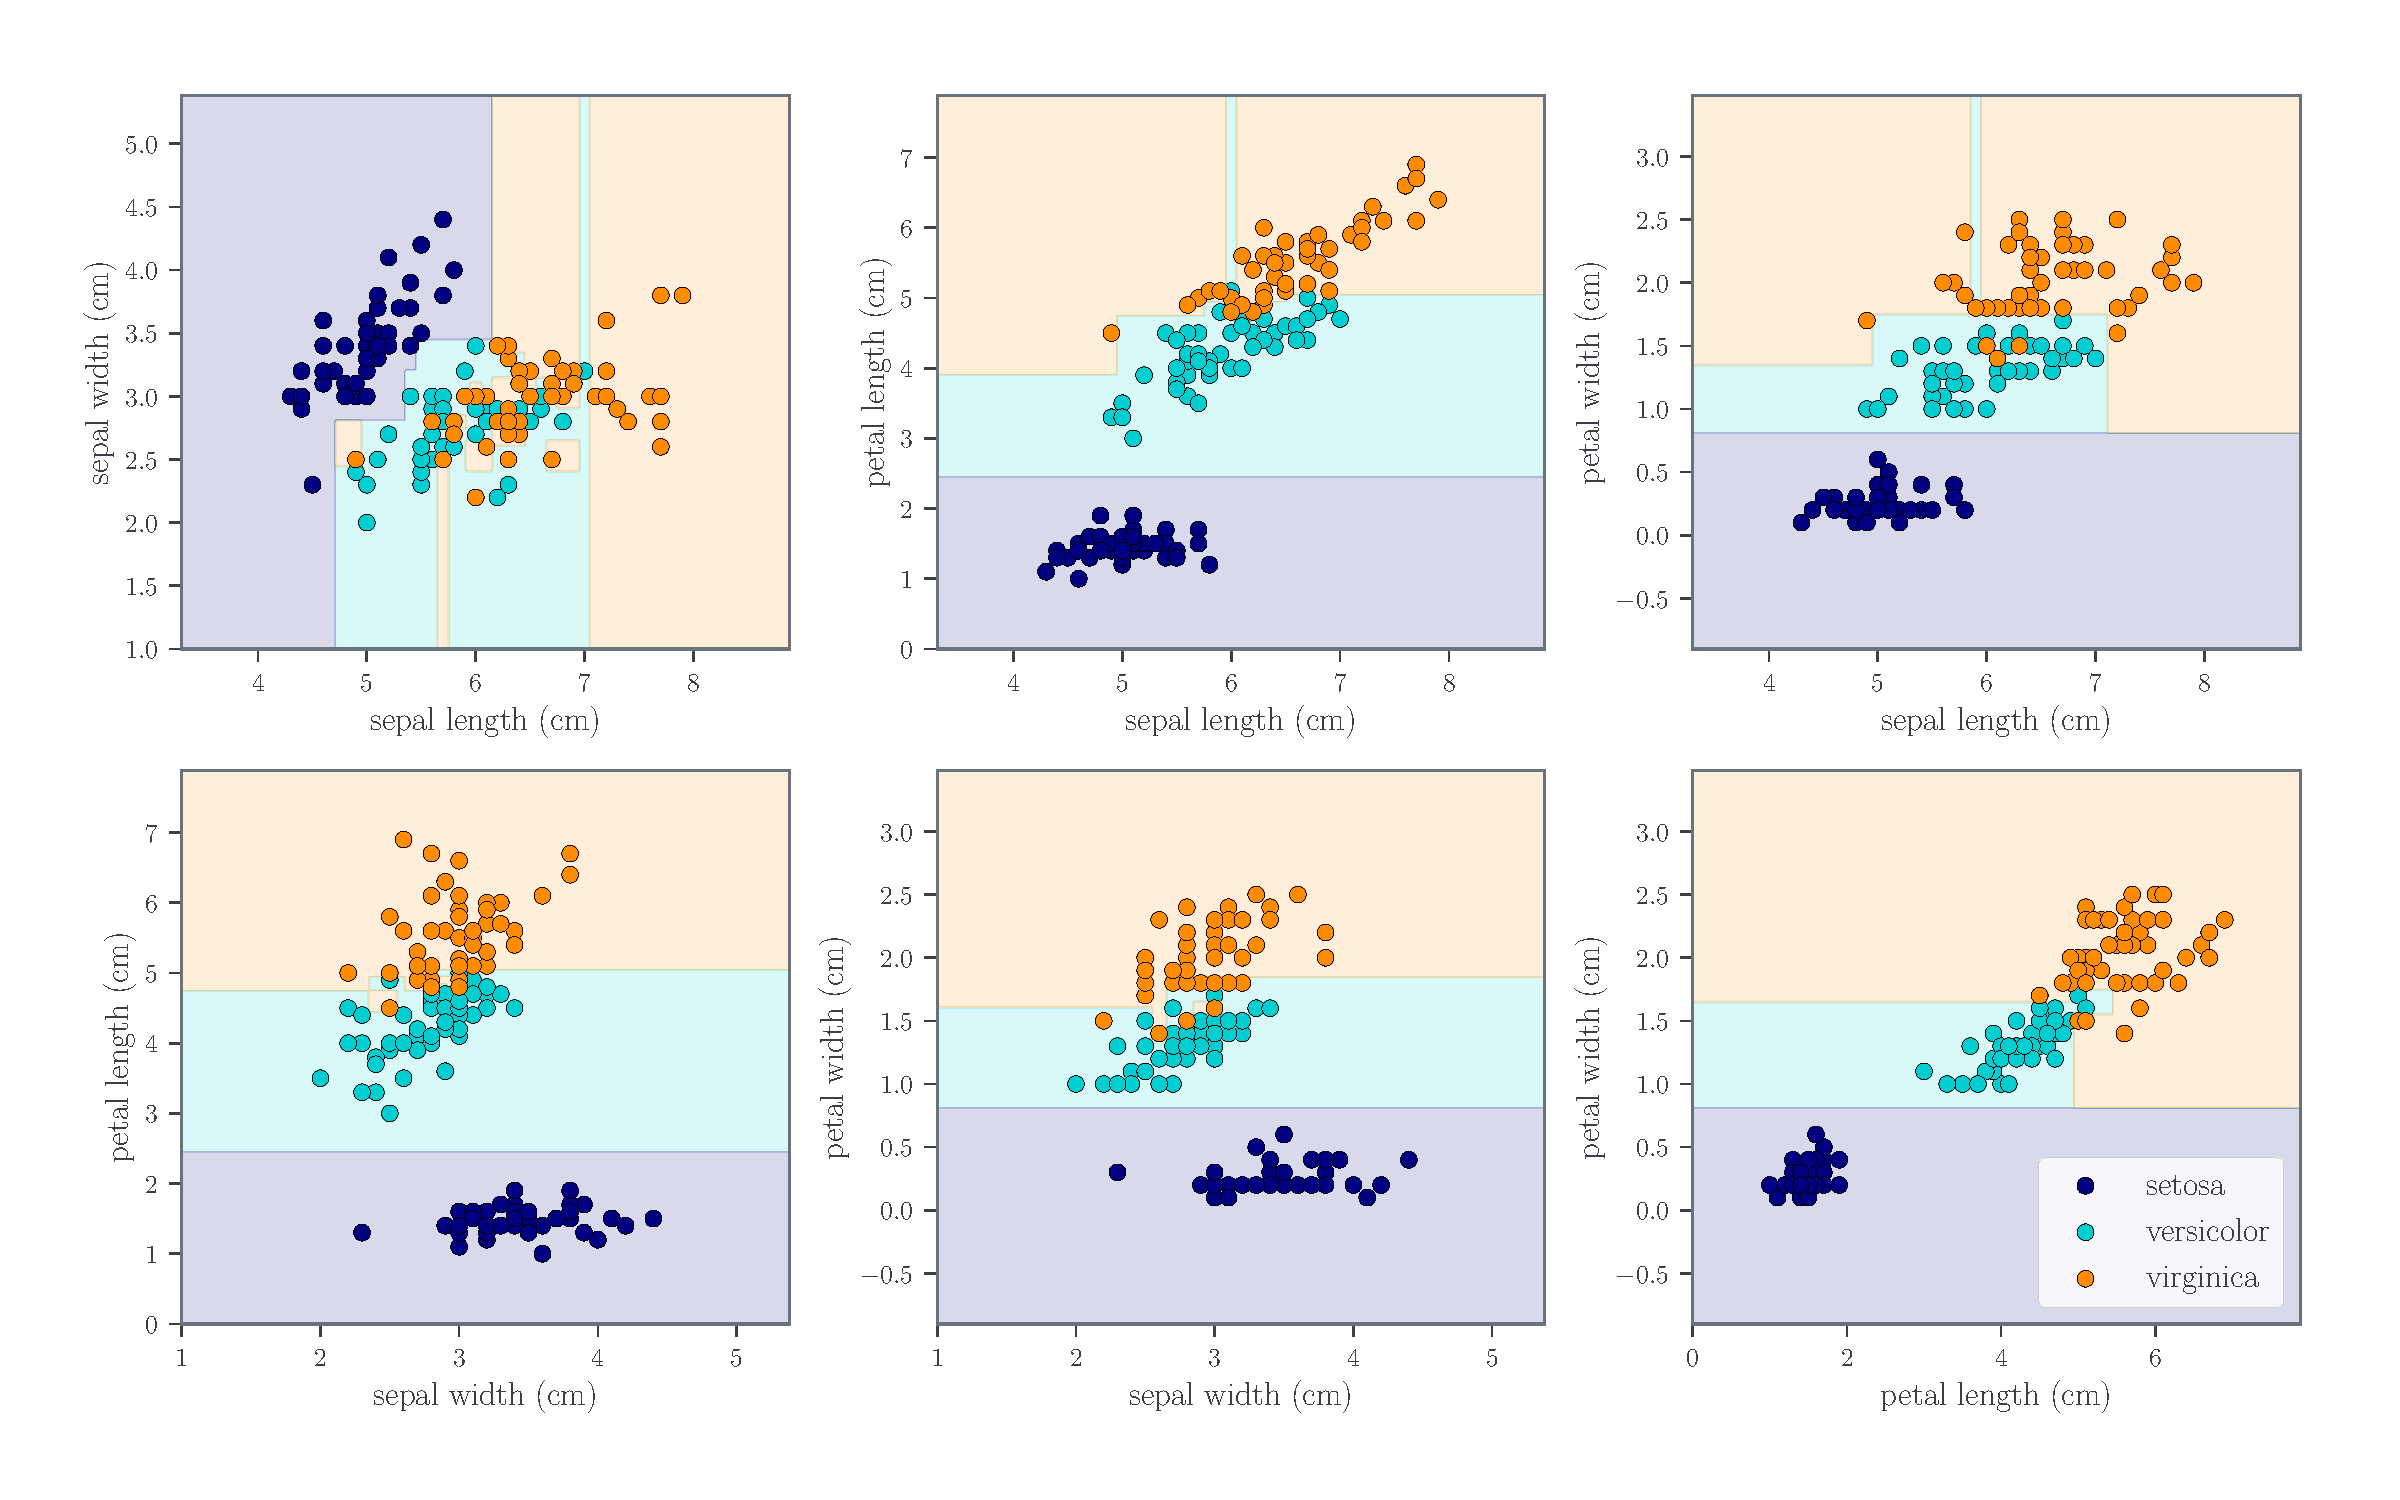
\includegraphics[width=\linewidth]{./img/tree_decision_surface.pdf}
\end{figure}

\subsubsection{Regression criteria}
For continuous target outcome, a common criteria is the \textbf{mean squared error}
\begin{equation}
\bar{y}_m = \frac{1}{N_m} \sum_{i\in N_m} y_i
\end{equation}
\begin{equation}
H(\mathcal{X}_m) = \frac{1}{N_m} \sum_{i\in N_m} (y_i - \bar{y}_m)^2
\end{equation}
\begin{figure}[h!]
	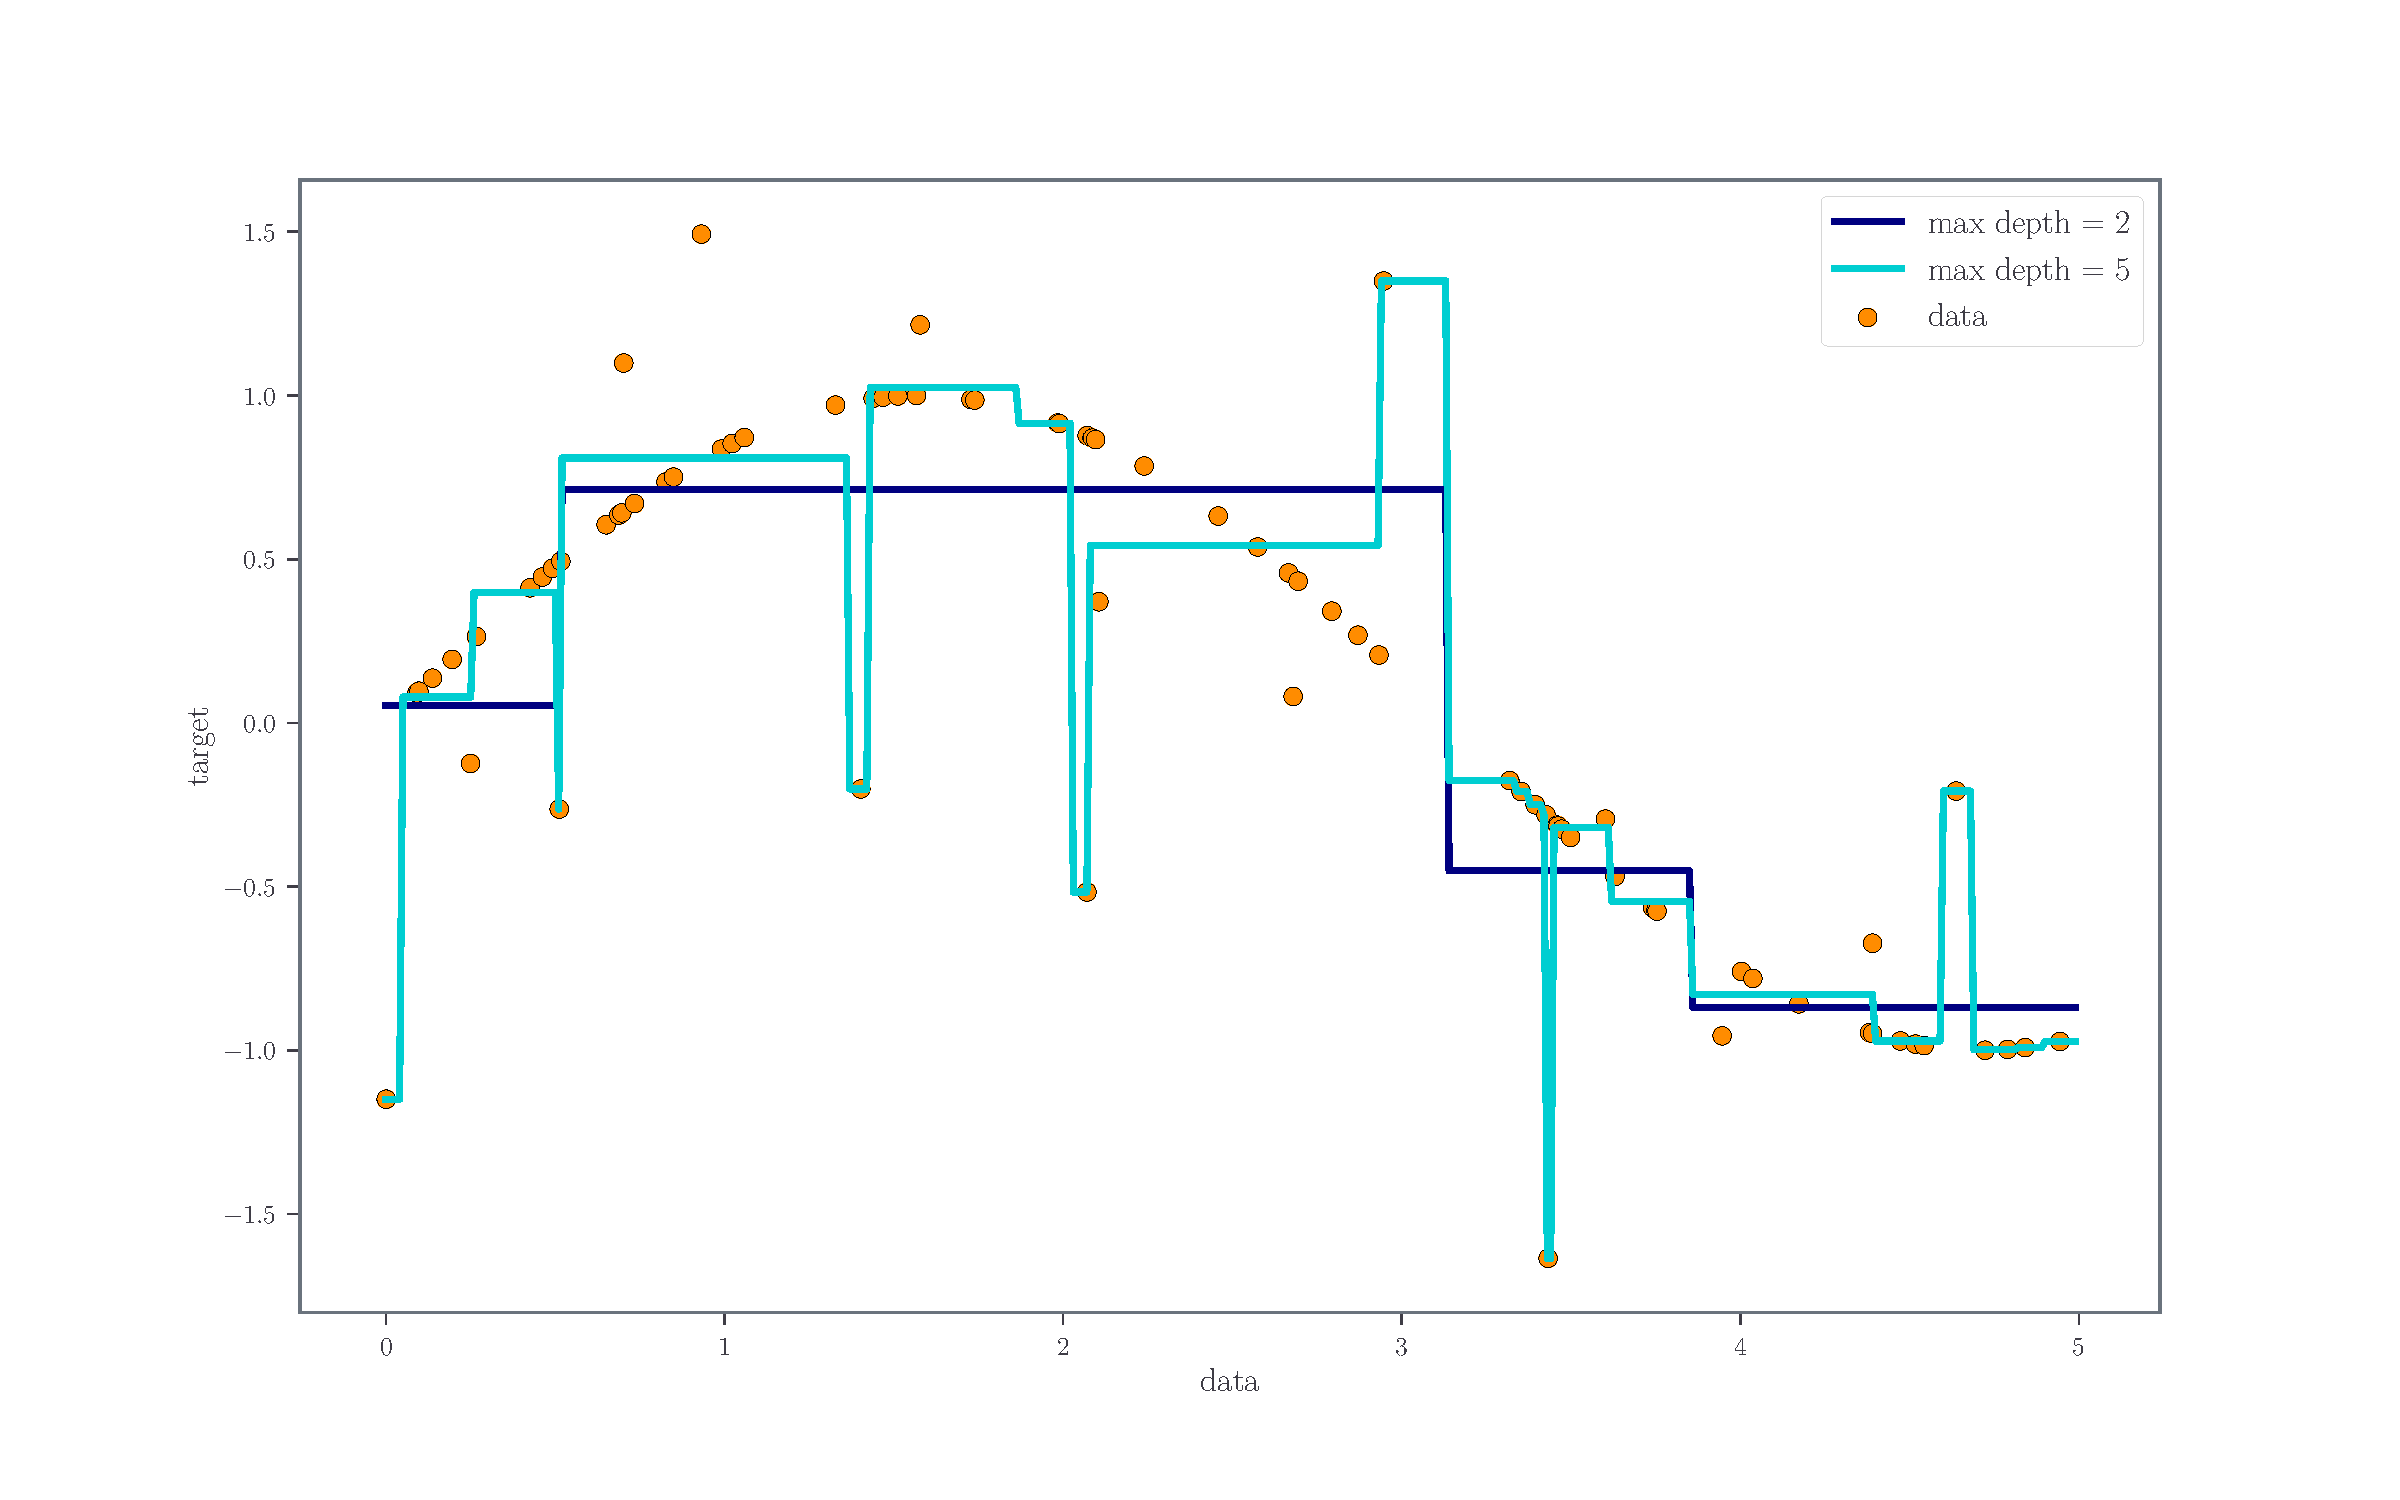
\includegraphics[width=\linewidth]{./img/tree_regression.pdf}
\end{figure}




\section{Ensemble Learning}
Decision trees are sensitive to the specific data on which they are trained. If the training data is changed (e.g. a tree is trained on a subset of the training data) the resulting decision tree can be quite different and in turn the predictions can be quite different.

The goal of \textbf{ensemble learning} is to combine the predictions of several base estimators built with a given learning algorithm in order to improve generalizability / robustness over any individual estimator. There are two categories:
\begin{itemize}
	\item \textbf{Averaging methods:} build several estimators independently and then average their predictions. on average, the combined estimator is better than any of the single base estimators because its variance decreases.
	\item \textbf{Boosting methods:} base estimators are built sequentially trying to reduce the bias of the combined estimator. The motivation is to combine several weak learners to a powerful ensemble.
\end{itemize}

\subsection{Averaging methods}
In statistics, \textbf{bootstrapping} is any test or metric that relies on random sampling with replacement. The basic idea of bootstrapping is that inference about a population from sample data, (sample $\rightarrow$ population), can be modelled by resampling the sample data and performing inference about a sample from resampled data, (resampled $\rightarrow$ sample).

\subsubsection{Boostrap aggregating}
Bootstrap aggregating, \textbf{bagging}, is a ensemble meta-algorithm designed to reduce the variance in statistical classification and regression algorithms to avoid overfitting. Bagging is the application of bootstrapping to a high-variance machine learning algorithm, typically decision trees.

Given a training set $X=x_i,\dots,x_N \in \mathcal{X}$ with resonse $Y=y_i,\dots,y_N \in \mathcal{Y}$ bagging repeatedly selects a random sample with replacement from the training set and fits trees to these samples. That is, for $b = 1, \dots, B$ sample $N$ examples with replacement from $\mathcal{D}$, denoted $X_b$, $Y_b$, and train a decision tree $f_b$ on $X_b$, $Y_b$.

After training, predition on $x_{new}$ can be made by averaging from all individual regression trees on $x_{new}$
\begin{equation}\
\hat{f} = \frac{1}{B} \sum_{b=1}^B f_b(x_{new})
\end{equation}
or by taking a majority vote in the case of classification trees.

This bootstrapping procedure leads to better model performance because it decreases the variance of the model, without increasing the bias. This means that while the predictions of a single tree are highly sensitive to noise in its training set, the average of many trees is not, as long as the trees are not correlated. Simply training many trees on a single training set would give strongly correlated trees (or even the same tree many times, if the training algorithm is deterministic); bootstrap sampling is a way of de-correlating the trees by showing them different training sets.


\subsubsection{Random Forest}
Trees that are grown very deep tend to learn highly irregular patterns: they overfit their training sets, i.e. have low bias, but very high variance. Random forests are a way of averaging multiple deep trees, trained on different parts of the same training set, with the goal of reducing the variance. This comes at the expense of an increase in the bias and some loss of interpretability, but generally greatly boosts the performance in the final model. In random forests, each tree in the ensemble is built from a sample drawn with replacement (i.e., a bootstrap sample) from the training set. 

In addition, when splitting a node during the construction of the tree, the split that is chosen is no longer the best split among all features. Instead, the chosen split is the best split among a random subset of the features.  Only a selection of the features is considered at each node split which decorrelates the trees in the forest.

The reason for doing this is the correlation of the trees in an ordinary bootstrap sample: if one or a few features are very strong predictors for the response variable (target output), these features will be selected in many of the $B$ trees, causing them to become correlated.

\begin{itemize}
	\item For classification a good default is: \verb|m = sqrt(n)|
	\item For regression a good default is: \verb|m = n/3|
\end{itemize}
where $m$ is the number of randomly selected features that can be searched at a split point and $k$ is the number of input variables.


\subsubsection{ExtraTrees}
Extremely randomized trees, or ExtraTrees are trained using bagging and the random subspace method, like in an ordinary random forest, but additionally the top-down splitting in the tree learner is randomized. Instead of computing the locally optimal feature/split combination (based on, e.g., information gain or the Gini impurity), for each feature under consideration, a random value is selected for the split. This value is selected from the feature's empirical range (in the tree's training set, i.e., the bootstrap sample).


As in random forests, a random subset of candidate features is used, but instead of looking for the most discriminative thresholds, thresholds are drawn at random for each candidate feature and the best of these randomly-generated thresholds is picked as the splitting rule. This usually allows to reduce the variance of the model a bit more, at the expense of a slightly greater increase in bias

Both methods are about the same, with the ET being a bit worse when there is a high number of noisy features (in high dimensional data-sets).


\subsubsection{Feature importance valuation}
The relative rank (i.e. depth) of a feature used as a decision node in a tree can be used to assess the relative importance of that feature with respect to the predictability of the target variable. Features used at the top of the tree contribute to the final prediction decision of a larger fraction of the input samples. The expected fraction of the samples they contribute to can thus be used as an estimate of the relative importance of the features.

By averaging those expected activity rates over several randomized trees one can reduce the variance of such an estimate and use it for feature selection.


\subsection{Boosting methods}
Boosting is a machine learning ensemble meta-algorithm for primarily reducing bias, and also variance in supervised learning, and a family of machine learning algorithms that convert weak learners to strong ones.

While boosting is not algorithmically constrained, most boosting algorithms consist of iteratively learning weak classifiers with respect to a distribution and adding them to a final strong classifier. When they are added, they are typically weighted in some way that is usually related to the weak learners' accuracy. After a weak learner is added, the data are reweighted: examples that are misclassified gain weight and examples that are classified correctly lose weight (some boosting algorithms actually decrease the weight of repeatedly misclassified examples, e.g., boost by majority and BrownBoost). Thus, future weak learners focus more on the examples that previous weak learners misclassified.

\subsubsection{AdaBoost}
The core principle of Adaptive Boosting, or AdaBoost, is to fit a sequence of weak learners (i.e., models that are only slightly better than random guessing, such as small decision trees) on repeatedly modified versions of the data. The predictions from all of them are then combined through a weighted majority vote (or sum) to produce the final prediction (boosting outcome). 

The data modifications at each boosting iteration consist of applying weights $w_1, w_2,\dots, w_N$ to each of the training samples. Initially, those weights are all set to $w_i = 1/N$, so that the first step trains a weak learner on the original data. For each successive iteration, the sample weights are individually modified and the learning algorithm is reapplied to the reweighted data. At a given step, those training examples that were incorrectly predicted by the boosted model induced at the previous step have their weights increased, whereas the weights are decreased for those that were predicted correctly. 

As iterations proceed, examples that are difficult to predict receive ever-increasing influence. Each subsequent weak learner is thereby forced to concentrate on the examples that are missed by the previous ones in the sequence.

\subsubsection{Gradient Boosted Trees}
Gradient Tree Boosting or Gradient Boosted Regression Trees (GBRT) is a generalization of boosting to arbitrary differentiable loss functions. GBRT is an accurate and effective off-the-shelf procedure that can be used for both regression and classification problems. 

The advantages of GBRT are
\begin{itemize}
\item Natural handling of data of mixed type (= heterogeneous features)
\item Predictive power
\item Robustness to outliers in output space (via robust loss functions)
\end{itemize}

The disadvantages of GBRT are:
\begin{itemize}
	\item Scalability, due to the sequential nature of boosting it can hardly be parallelized.
\end{itemize}

\subsection{XGBoost}



\section{Unsupervised Learning}

\subsection{Cluster Analysis}
\textit{Cluster analysis} or \textit{clustering} is the task of grouping a set of objects in such a way that objects in the same group (called a cluster) are more similar (in some sense) to each other than to those in other groups (clusters).

\subsection{Principal Component Analysis (PCA)}
PCA is mathematically defined as an orthogonal linear transformation that transforms the data to a new lower-dimensional coordinate system such that the greatest variance by some projection of the data comes to lie on the first coordinate (called the first principal component), the second greatest variance on the second coordinate, and so on.



Normalization is important in PCA since it is a variance maximizing exercise. It projects your original data onto directions which maximize the variance\footnote{https://stats.stackexchange.com/questions/69157/why-do-we-need-to-normalize-data-before-principal-component-analysis-pca}. 

https://stackoverflow.com/questions/31909945/obtain-eigen-values-and-vectors-from-sklearn-pca

https://stackoverflow.com/questions/22984335/recovering-features-names-of-explained-variance-ratio-in-pca-with-sklearn

Technically, PCA is used to find the Eigenvalues $\lambda_j$ und Eingenvectors $\nu_j$ of the data correlation matrix $\Sigma = Y^T Y$, where $Y = X - \mu_X$ and $X$ is an $N \times K$ matrix of data points. $K$ corresponds to the number of features.


\section{Model Selection}

\subsection{Cross Validation}
Learning the parameters of a prediction function and testing it on the same data is a methodological mistake: a model that would just repeat the labels of the samples that it has just seen would have a perfect score but would fail to predict anything useful on yet-unseen data. This situation is called overfitting. To avoid it, it is common practice when performing a (supervised) machine learning experiment to hold out part of the available data as a test set.

When evaluating different settings (“hyperparameters”) for estimators there is still a risk of overfitting on the test set because the parameters can be tweaked until the estimator performs optimally. This way, knowledge about the test set can “leak” into the model and evaluation metrics no longer report on generalization performance. To solve this problem, yet another part of the dataset can be held out as a so-called “validation set”: training proceeds on the training set, after which evaluation is done on the validation set, and when the experiment seems to be successful, final evaluation can be done on the test set.

However, by partitioning the available data into three sets, we drastically reduce the number of samples which can be used for learning the model, and the results can depend on a particular random choice for the pair of (train, validation) sets.

A solution to this problem is a procedure called cross-validation (CV for short). A test set should still be held out for final evaluation, but the validation set is no longer needed when doing CV. In the basic approach, called k-fold CV, the training set is split into k smaller sets (other approaches are described below, but generally follow the same principles). The following procedure is followed for each of the k “folds”:

\begin{itemize}
	\item A model is trained using k-1 of the folds as training data;
	\item the resulting model is validated on the remaining part of the data (i.e., it is used as a test set to compute a performance measure such as accuracy).
\end{itemize}
The performance measure reported by k-fold cross-validation is then the average of the values computed in the loop. This approach can be computationally expensive, but does not waste too much data (as it is the case when fixing an arbitrary test set), which is a major advantage in problem such as inverse inference where the number of samples is very small.

\subsection{Estiamtion Accuracy Measurements}
sklearn precision recall, receiver operating characteristic

\subsubsection{In sample vs out of sample error}
\textit{In sample error} is the error rate from the same data set used for building a predictor, also referred to as resubstitution error.

\textit{Out of sample error} is the error rate that stems from predicting new data with a trained predictor, also referred to as generaluzation error.

\subsubsection{Precision-Recall}


\subsubsection{Receiver Operating Characteristic}
A receiver operating characteristic (ROC), or simply ROC curve, is a graphical plot which illustrates the performance of a binary classifier system as its discrimination threshold is varied. It is created by plotting the fraction of true positives out of the positives (TPR = true positive rate) vs. the fraction of false positives out of the negatives (FPR = false positive rate), at various threshold settings. TPR is also known as sensitivity, and FPR is one minus the specificity or true negative rate.

This means that the top left corner of the plot is the “ideal” point - a false positive rate of zero, and a true positive rate of one. This is not very realistic, but it does mean that a larger area under the curve (AUC) is usually better.

The “steepness” of ROC curves is also important, since it is ideal to maximize the true positive rate while minimizing the false positive rate.

This example shows the ROC response of different datasets, created from K-fold cross-validation. Taking all of these curves, it is possible to calculate the mean area under curve, and see the variance of the curve when the training set is split into different subsets. This roughly shows how the classifier output is affected by changes in the training data, and how different the splits generated by K-fold cross-validation are from one another.

\begin{figure}[h!]
	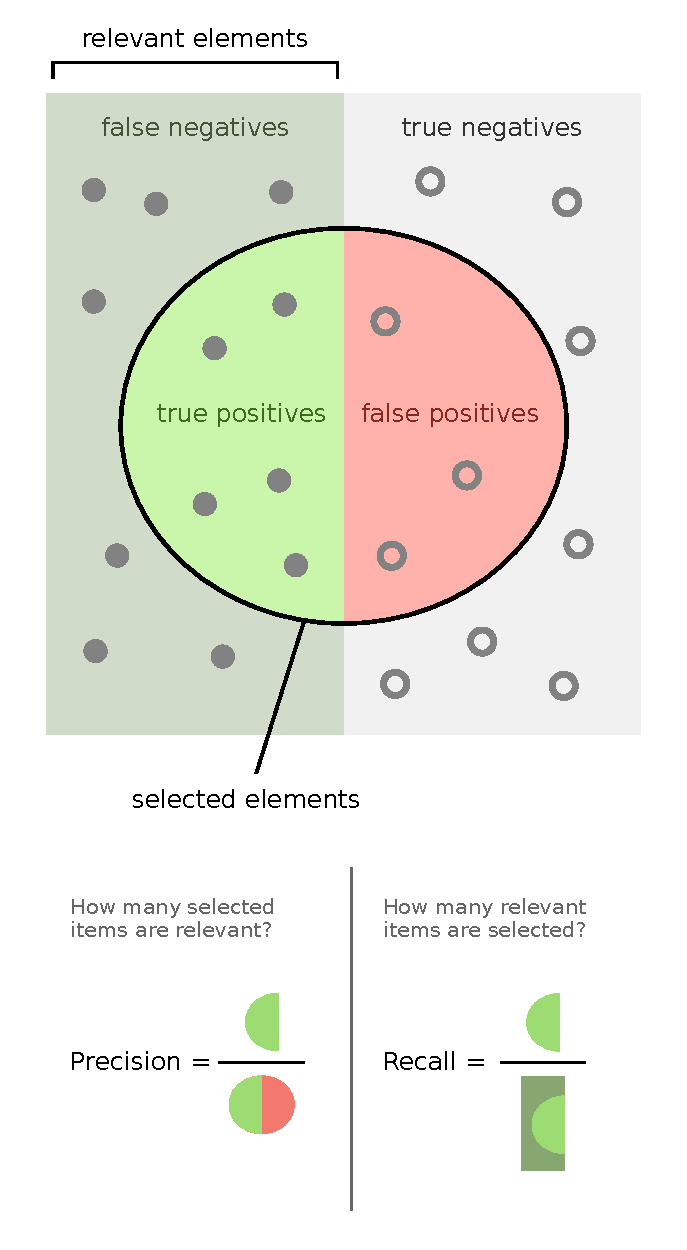
\includegraphics{./img/Precisionrecall.pdf}
\end{figure}




\section{Artificial Neural Networks}

\subsection{Artificial Neuron}

\subsection{Perceptron Learning}
The \textit{Perceptron} is an algorithm for learning a binary classifier: a mapping function $\text{y}=f(\text{x})$ of a real-valued input (vector) x to a binary output or target y
\begin{equation}
f(\text{x}) \ = \ \begin{cases}
0 & \text{if} \ \omega \cdot \text{x} + \text{b} \\
1 & \text{otherwise}
\end{cases}
\end{equation}
where $\omega$ is a real-valued vector of weights, $\omega \cdot \text{x}$ is the dot product $\sum_{i=1}^N \omega_i x_i$, $N$ is the total number of inputs to the neuron, and b is the \textit{bias}. The bias shifts the decision boundary away from the origin and does not depend on any input value.


http://cs229.stanford.edu/notes/cs229-notes2.pdf

area under curve

neural networks

expection maximization

risk management

bayes krankheit bespiel verstehen


\section{Blockchain}
A \textit{Blockchain} is an \textit{immutable}, \textit{sequential} chain of records called \textit{Blocks}. They can contain transactions, files or any other data which are chained together using \textit{hashes}.

Each Block has an \textit{index}, a \textit{timestamp} (in Unix time), a \textit{list of transactions}, a \textit{proof} and the \textit{hash of the previous block}. The hash of the previous block is what gives the Blockchain its immutability. TH first block in the chain is called \textit{genesis} block as it has no predecessors

\subsection{Proof of work algoritj}
A \textit{Proof of Woork} algorithm (PoW) is the process of creating or \textit{mining} a new block on the blockchain. The goal of the PoW is to discover a number that is computationally difficult to find, but at the same time easy to verify by anyone in the network.

In Bitcoin, the PoW algorithm is called \textit{HashCash}. In general, the difficulty is determined by the number of characters searched for in a string. The miners are then rewarded for their solution by receiving a coin -  in a transaction.


markov process

https://hackernoon.com/learn-blockchains-by-building-one-117428612f46

\section{Data Warehousing}
acid

etl 

\section{Time Series Analysis}


\end{document}